% =====================================================================
%  Chapter 8 — Shape as the Geometry \idxw{Volume} Is Built From
% =====================================================================

\chapter{Shape as the Geometry Volume Is Built From}
\label{ch:shape-geometry}

The volume\idx{Volume} of a body is not observable. What is observable is its projected
area, and the volume\idx{Volume} has to be constructed from that projection on the
assumption that the body is convex. This chapter is about that construction:
why it is unavoidable, what it costs, and what the one measurement in the
record that bypassed it actually found.

\section{Why volume cannot be observed}

A shape model is a three-dimensional object, and a shape model is not a
measurement. It is an inversion: a set of constraints on the body's
silhouette, or on its brightness as it rotates, combined with an assumed
geometry, yields a body.

The distinction matters for the energy chain, because \eqref{eq:energy} needs
a volume\idx{Volume} and not an area. The projected area of a body at a given aspect
angle is a measurement. The volume behind that projection is not. The
conversion from one to the other is the convex-hull assumption, and it is
the assumption that a resolved image cannot avoid either --- but it can
\emph{measure} it, by imaging the body from more than one aspect, or by
using the rotation to image it from many.

For a convex body, the convex hull of the projected silhouette is the body,
and the volume is exact. For a non-convex body, the convex hull is larger
than the body, and the error is one-sided: it always overstates the volume.

\section{What the record contains}

The measurement record of asteroid shapes by interferometry consists, almost
entirely, of one result, and it is worth reading in detail because it is
unique in every respect that matters.

On 15 May 2017 the asteroid (372) Palma occulted the radio galaxy
0141+268. The shadow of the asteroid crossed the Very Long Baseline Array
station at Brewster, Washington, and six \idxw{VLBA} antennas recorded it. At the
observing wavelength of 4.2 centimetres, with the asteroid's radius near
95 kilometres and its distance at 3.436 astronomical units, the Fresnel
number was 0.43 --- which means the diffraction pattern fell in the
Fraunhofer regime and was observable on the Earth.

The measurement retrieved both the amplitude and the phase of the diffracted
electromagnetic wave. It is the first astronomical measurement of the phase
shift caused by diffraction by an asteroid, and the maximum phase shift is
directly sensitive to the effective diameter.

\begin{table}[!htbp]
\centering
\small
\caption{The 2017 radio occultation of (372) Palma: what was measured and
what it returned.}
\label{tab:palma}
\begin{tabularx}{\textwidth}{@{}P{2.57in}Y@{}}
\toprule
\rowcolor{panel}
\textbf{Quantity} & \textbf{Value} \\
\midrule
Technique & radio occultation\idx{Radio occultation}, six VLBA\idx{VLBA} antennas, 4.2 cm, 6.996 GHz \\
\rowcolor{panel}
Baselines to the Brewster station & 1,200 to 2,300 km \\
\idxw{Fresnel number} & 0.43, Fraunhofer regime \\
\rowcolor{panel}
Effective diameter, all silhouette models & \(192.1 \pm 2.3\) km \\
Effective diameter, circular-disk fit & \(192.1 \pm 4.8\) km \\
\rowcolor{panel}
Maximum phase shift & \(76.4 \pm 2.5\) degrees \\
Cross-check, thermal mid-infrared & \(191.1 \pm 2.7\) km and
\(186.5 \pm 6.3\) km \\
\rowcolor{panel}
Roundness, ratio of inscribed to circumscribed circle & mean 0.866, standard
deviation 0.093 \\
Departure from a circle & 10 to 20 per cent \\
\bottomrule
\end{tabularx}
\end{table}

Three things in \tabref{tab:palma} matter for the rest of the book.

The first is the scale. The measured object is 192 kilometres across. The
class this book is about is 50 to 140 metres across, so Palma is more than
a thousand times wider in diameter and more than a billion times larger in
volume. Any statement about the feasibility of asteroid interferometry has
to be read with that ratio in mind.

The second is the shape. The silhouette is slightly elongated and has a
concave edge, and the roundness distribution --- built from 24,000 random
contiguous silhouettes fitted to the observed amplitude and phase curves ---
has a mean of 0.866 with a standard deviation of 0.093, and gives a
departure from a perfect circle of 10 to 20 per cent with the roundness
bounded below at 0.63 with ninety-five per cent confidence. The earlier
arXiv abstract of the same study gave the departure as \(26 \pm 13\) per
cent; both figures are carried here because both were published, and the
conclusion is the same either way.

The third is the epilogue. The study notes that although the more than
1,600 astrometric observations of Palma span more than 120 years, the
addition of a single radio interferometric occultation measurement had a
non-negligible effect on the uncertainties of the orbital elements and
reduced the uncertainty of the ephemerides by an order of magnitude. One
measurement, one night, and the long-term ephemeris improved by a factor of
ten. That is the character of the observation this book is proposing.

\section{The scale of the problem, restated}

\begin{figure}[!htbp]
\centering
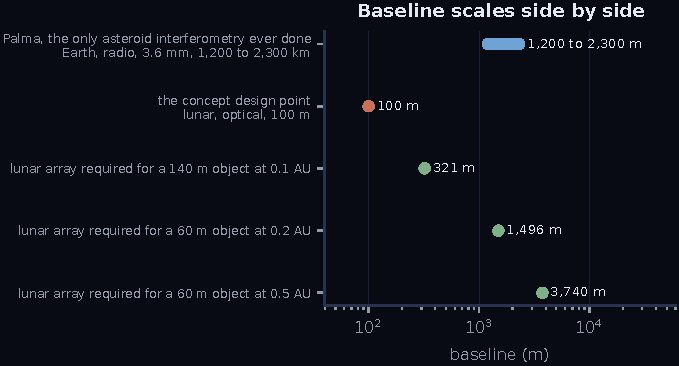
\includegraphics[width=\textwidth]{../figures/fig_scale.pdf}
\caption{Baseline scales side by side. The only asteroid interferometry ever
performed used terrestrial baselines of 1,200 to 2,300 kilometres at radio
wavelengths, on a target 192 kilometres wide. The baselines an optical
shape imager needs for the small class are one to two orders of magnitude
shorter, but they have to be held to a stability the ground cannot hold.}
\label{fig:scale}
\end{figure}

\figref{fig:scale} sets the two scales against each other, and the
comparison is deliberately framed in the most favourable way available to the
existing technique. Palma's measurement used the largest terrestrial
baselines there are, at radio wavelengths where the coherence requirements
are mild, on a target three orders of magnitude larger than the class this
book concerns, and it worked.

The optical problem is different in kind rather than in degree. A
radio-interferometric image of an unresolved body at 4.2 centimetres is
obtained by measuring the amplitude and phase of a diffraction pattern; an
optical interferometric image of a resolved body at 750 nanometres requires
the fringe visibility of a limb profile to be measurable, which requires the
baseline to be matched to the body's angular size rather than to exceed it.
Chapter 20 works through that condition, and it is the reason the concept
literature's hundred-metre baseline does not do what the book needs.

\section{What this means for the energy chain}

The chain can now be written out in the form the rest of the book uses.

\begin{table}[!htbp]
\centering
\small
\caption{From a resolved image to an energy, with the assumption at each
step made explicit.}
\label{tab:shape-to-energy}
\begin{tabularx}{\textwidth}{@{}P{1.20in}P{1.36in}Y@{}}
\toprule
\rowcolor{panel}
\textbf{Step} & \textbf{Quantity produced} & \textbf{Assumption} \\
\midrule
Resolved image & projected area at the epoch & none; this is a measurement \\
\rowcolor{panel}
Projection to volume & volume & convexity\idx{Convexity}, unless the rotation supplies
multiple aspects \\
Volume to mass & mass & bulk density \\
\rowcolor{panel}
Mass to energy & energy & impact speed, which is well determined \\
Energy to hazard class & Torino level & the scale's own definitions \\
\bottomrule
\end{tabularx}
\end{table}

The middle row is where a resolved image earns its place. It replaces a
model choice --- the thermal beaming parameter, or the convexity\idx{Convexity} of the
inversion --- with a measurement, and it is the only step in the chain that
a resolved image can close without any other instrument's help. The row
below it is the one that requires an encounter, and Chapter 7 has argued
that the same encounter supplies it.

\begin{keytakeaways}
\item A volume cannot be observed; it is constructed from a projection, and
the construction assumes convexity.
\item The convex-hull error is one-sided: it always overstates the volume.
\item The only asteroid silhouette ever measured by interferometry is
(372) Palma, by radio occultation\idx{Radio occultation} with the VLBA\idx{VLBA}, and it found a body 192
kilometres across whose silhouette departs from a circle by 10 to 20 per
cent.
\item A single such measurement reduced that object's long-term ephemeris
uncertainty by an order of magnitude.
\end{keytakeaways}
